\begin{enumerate}

\item Let us label the output of the LFSR $110100100001010$ as

\[s_0 || s_1 || s_2 || ... || s_{14} \]

where $s_i$ is the $i$th bit of the sequence of bits generated by our LFSR. Then

\begin{align*}
\begin{pmatrix}
s_5 \\ s_6 \\ s_7 \\ s_8 \\ s_9 
\end{pmatrix}
&= 
\begin{pmatrix}
s_0 & s_1 & s_2 & s_3 & s_4 \\
s_1 & s_2 & s_3 & s_4 & s_5 \\
s_2 & s_3 & s_4 & s_5 & s_6 \\
s_3 & s_4 & s_5 & s_6 & s_7 \\
s_4 & s_5 & s_6 & s_7 & s_8 \\
\end{pmatrix} 
\begin{pmatrix}
c_0 \\ c_1 \\ c_2 \\ c_3 \\ c_4
\end{pmatrix} 
\end{align*}

where $c_i$ is the $i$th connection coefficient. Substituting in our values and
solving for the $c_i$s, we have that

\begin{align*}
\Rightarrow 
\begin{pmatrix}
c_0 \\ c_1 \\ c_2 \\ c_3 \\ c_4
\end{pmatrix}
&=
\begin{pmatrix}
1 & 1 & 0 & 1 & 0 \\
1 & 0 & 1 & 0 & 0 \\
0 & 1 & 0 & 0 & 1 \\
1 & 0 & 0 & 1 & 0 \\
0 & 0 & 1 & 0 & 0 
\end{pmatrix}^{-1}
\begin{pmatrix} 0 \\  1 \\ 0 \\ 0 \\ 0 \end{pmatrix} \\
&=
\begin{pmatrix}
0 & 1 & 0 & 0 & 1 \\
1 & 0 & 0 & 1 & 0 \\
0 & 0 & 0 & 0 & 1 \\
0 & 1 & 0 & 1 & 1 \\
1 & 0 & 1 & 1 & 0
\end{pmatrix}
\begin{pmatrix} 0 \\  1 \\ 0 \\ 0 \\ 0 \end{pmatrix} \\
&=
\begin{pmatrix} 1 \\  0 \\ 0 \\ 1 \\ 0 \end{pmatrix}
\end{align*}.

This means that $c_0, c_3$ are 1 with $c_1, c_2, c_4$ being 0.

\item See included diagram below.
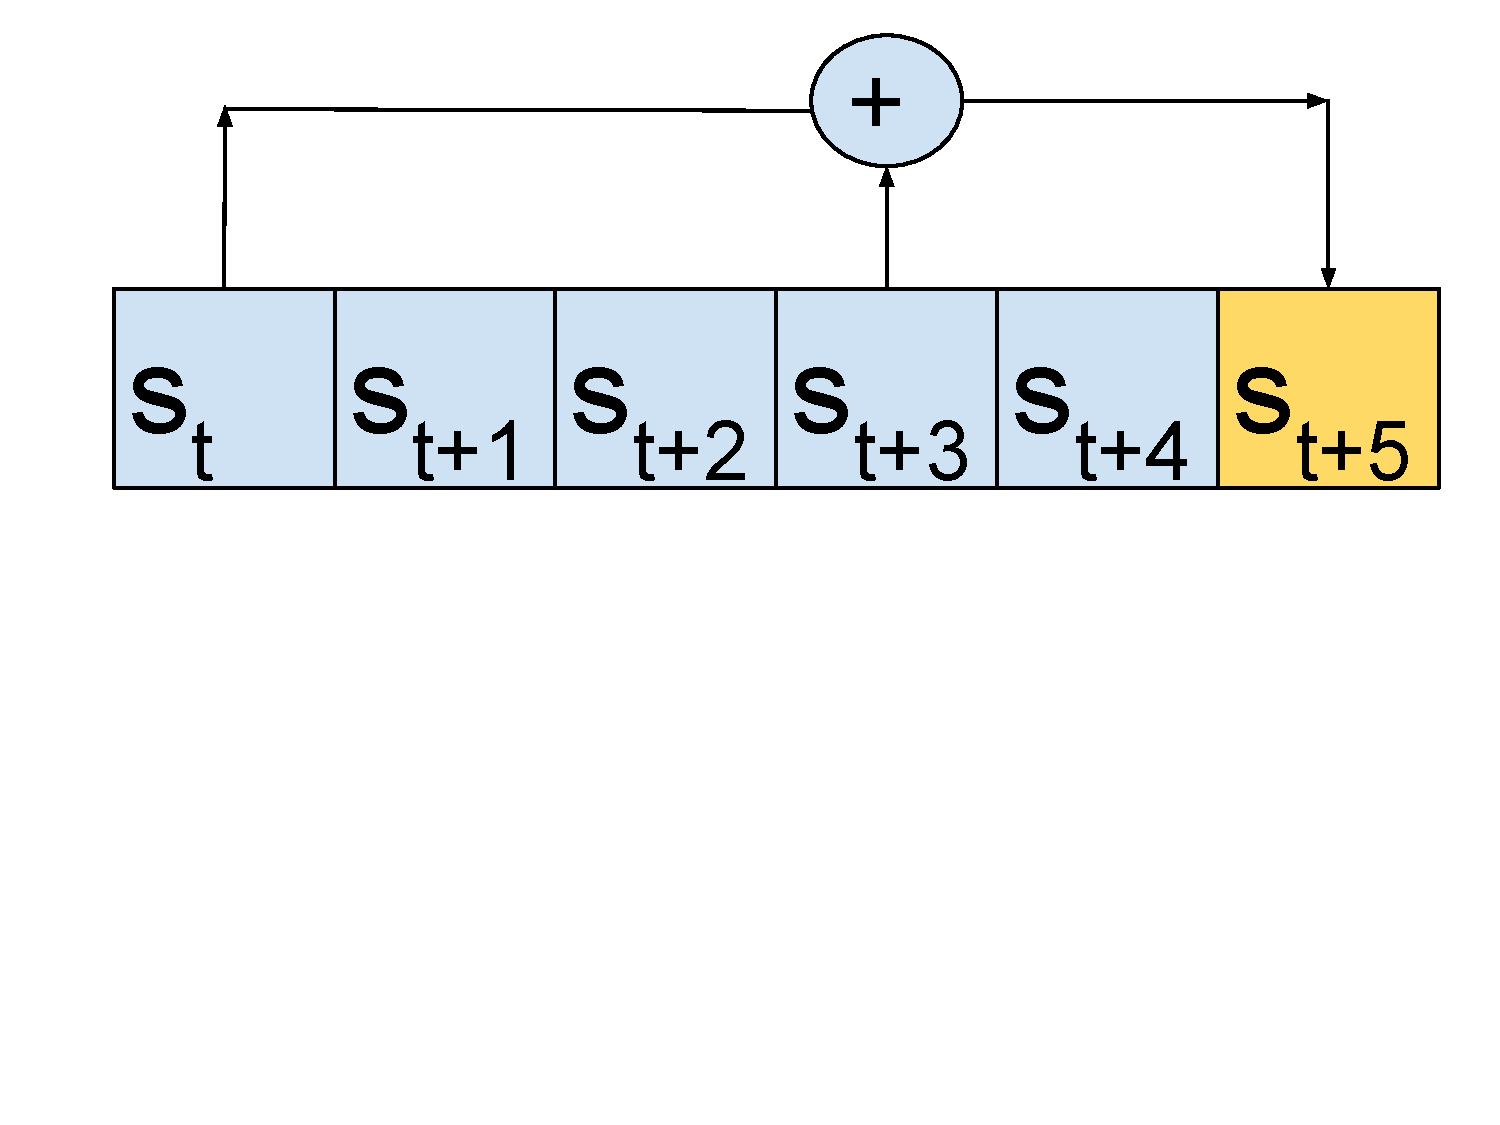
\includepdf[pages={1}]{lfsr.pdf}

\item One characteristic polynomial would be $F(X) = X^5 + X^3 + 1$.

\item We do this by contradiction. Since L is the length of the shortest LFSR
that can produce this sequence, we know that this LFSR has a minimal polynomial of
degree L. We now show that if the first L states are linearly dependent,
then the LFSR has a minimal polynomial of length L-1.

If states $S_0, S_1, \dots, S_{L-1}$ are linearly dependent, then there exists
$a_0, a_1, \dots, a_{L-1}$ not all zero such that

\[a_0S_0 + a_1 S_1 + \dots + a_{L-1} S_{L-1} = 0 \]

If $A$ is the matrix that represents the LFSR, then we have that

\[a_0S_0 + a_1 A S_1 + \dots + a_{L-1} A^{L-1} S_0 = \left(a_0 + a_1 A +
\dots + a_{L-1} A^{L-1} \right) S_0 = 0 \]

as each state $S_i$ is derived from the previous state $S_{i-1}$ by an
application of $A$.

If $S_0=0$, then all following states will also be zero as
they are simply linear combinations of the bits of $S_0$. This would means that
which means that $L$ would be $1$, as this would be the smallest LFSR capable of
making the zero sequence. If there's only one state, then it's linearly
independent by default.

If $S_0 \neq 0$, then we have that

\[a_0 + a_1 A + \dots + a_{L-1} A^{L-1} = 0 \]. Since some $a_i$ are non-zero,
this defines a non-zero polynomial $f(X) = a_0 + a_1 X + \dots + a_{L-1}
X^{L-1}$, As $f(A) = 0$, $f$ is a characteristic polynomial of $A$ and therefore
of the LFSR.  But, we know that the minimum polynomial of the LFSR and therefore
$A$ has degree $L$, whereas $deg(f) \leq L - 1$. Contradiction! Therefore the
first L states are linearly independent.

\end{enumerate}
